\chapter{Text Classification}

\marginnote{Aarne and Thompson were two folklorists, who invented and perfected the motif-based classification system of folk tales. This system has been in place since 1910 and is commonly used in comparative folkloristics. The final U in ATU stands for Uther, who was the last to update the index in 2004.}Grimm's tales corpus contains the attribute for Aarne-Thompson type (ATU). This is the index of folk-tale motifs and the tale have a high-level (genre) and a mid-level ATU type (subgenre).

Could we perhaps predict the ATU type based on the content of the tale? Let us see.

First, we need a target variable. This is the feature we are trying to predict, in our case an ATU type. We also need a numerical representation of each document - something we already have from the \widget{Bag of Words}.

\vspace{-0.2cm}
\begin{figure*}[h]
  \centering
  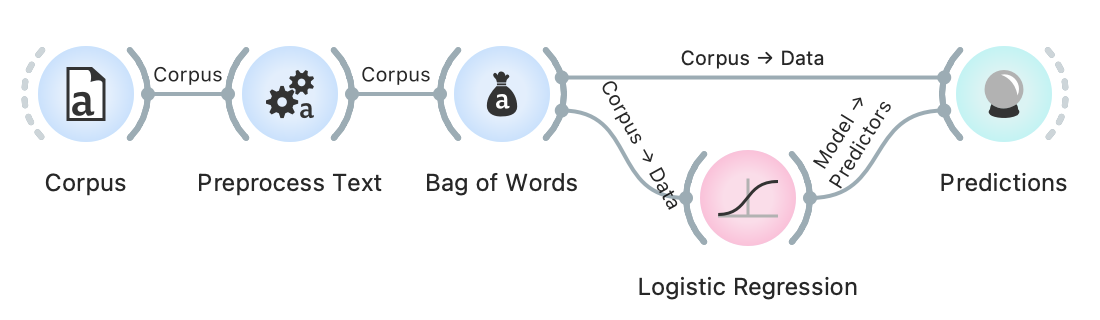
\includegraphics[width=0.8\linewidth]{workflow.png}%
  \caption{$\;$}
\end{figure*}
\vspace{-0.3cm}

Now we will build a predictive model. A predictive model considers tokens (words) and predicts the target variable (ATU Topic). Every model also needs a learner, which is a method on how to consider the tokens. A commonly used classifier in text mining is \widget{Logistic Regression}.

In Predictions, we can see a column with predicted values from Logistic Regression. Seems like our model got most of the tale types right.

\vspace{-0.2cm}
\begin{figure*}[h]
  \centering
  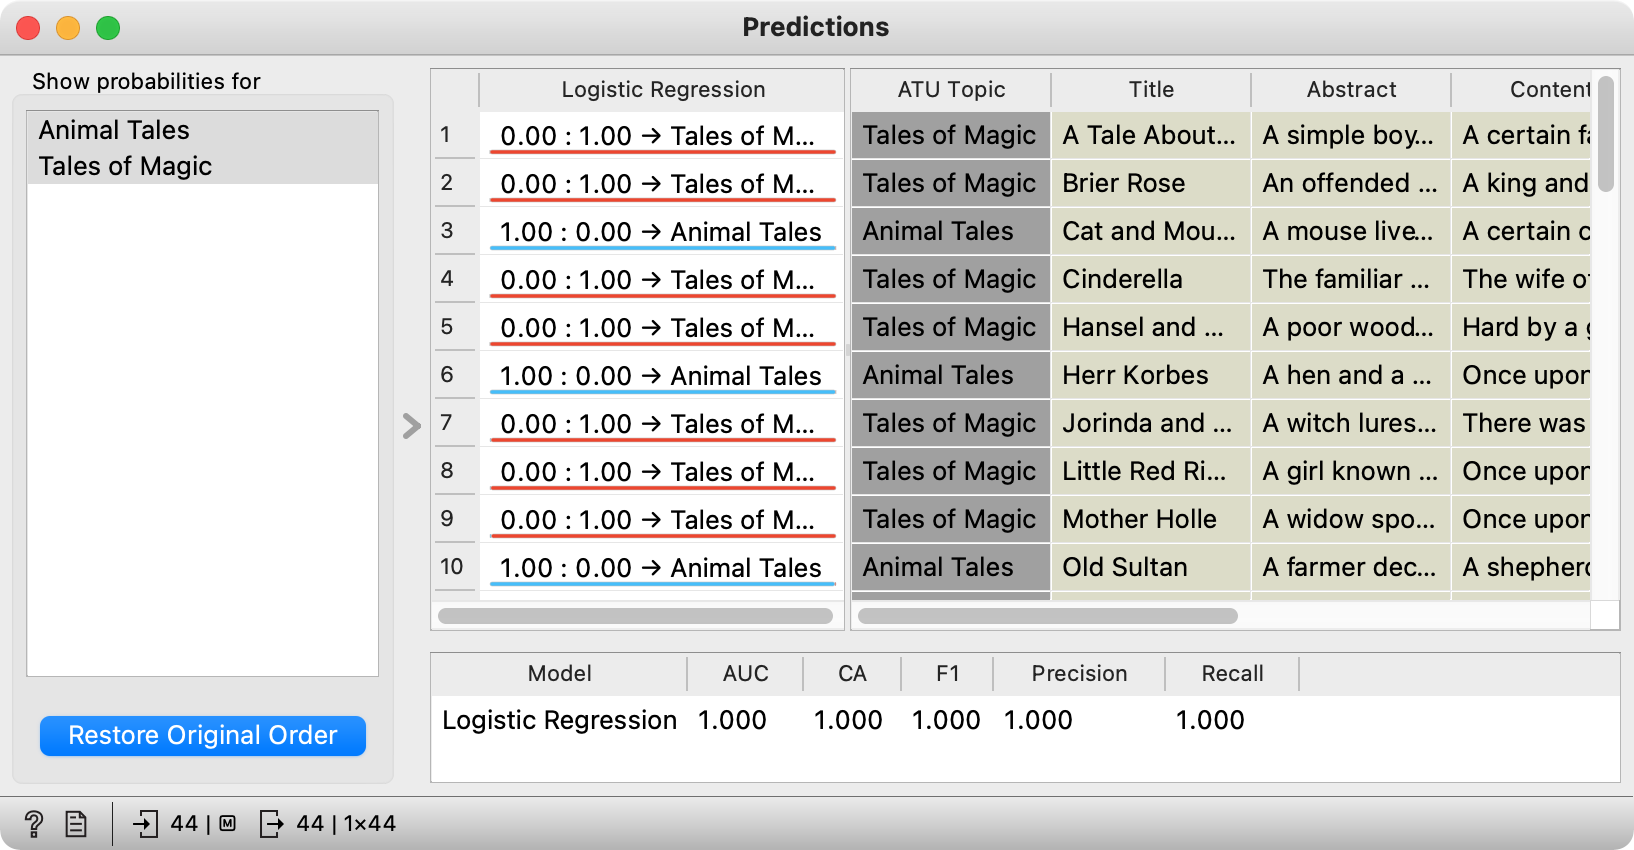
\includegraphics[width=0.9\linewidth]{predictions.png}%
  \caption{$\;$}
\end{figure*}
\vspace{-0.3cm}
